\newpage
\section{Test 7}
\label{Sec:test_7}

In the seveth test setting rover is dropped onto the horizontal plane.
An obstacle in the form of a horizontal step of height $0.1$ $m$ has been set in front of the rover.
At certain point rover starts moving towards the step and crosses it mounting on the higher plane.

\begin{figure}[H]
  \centering
    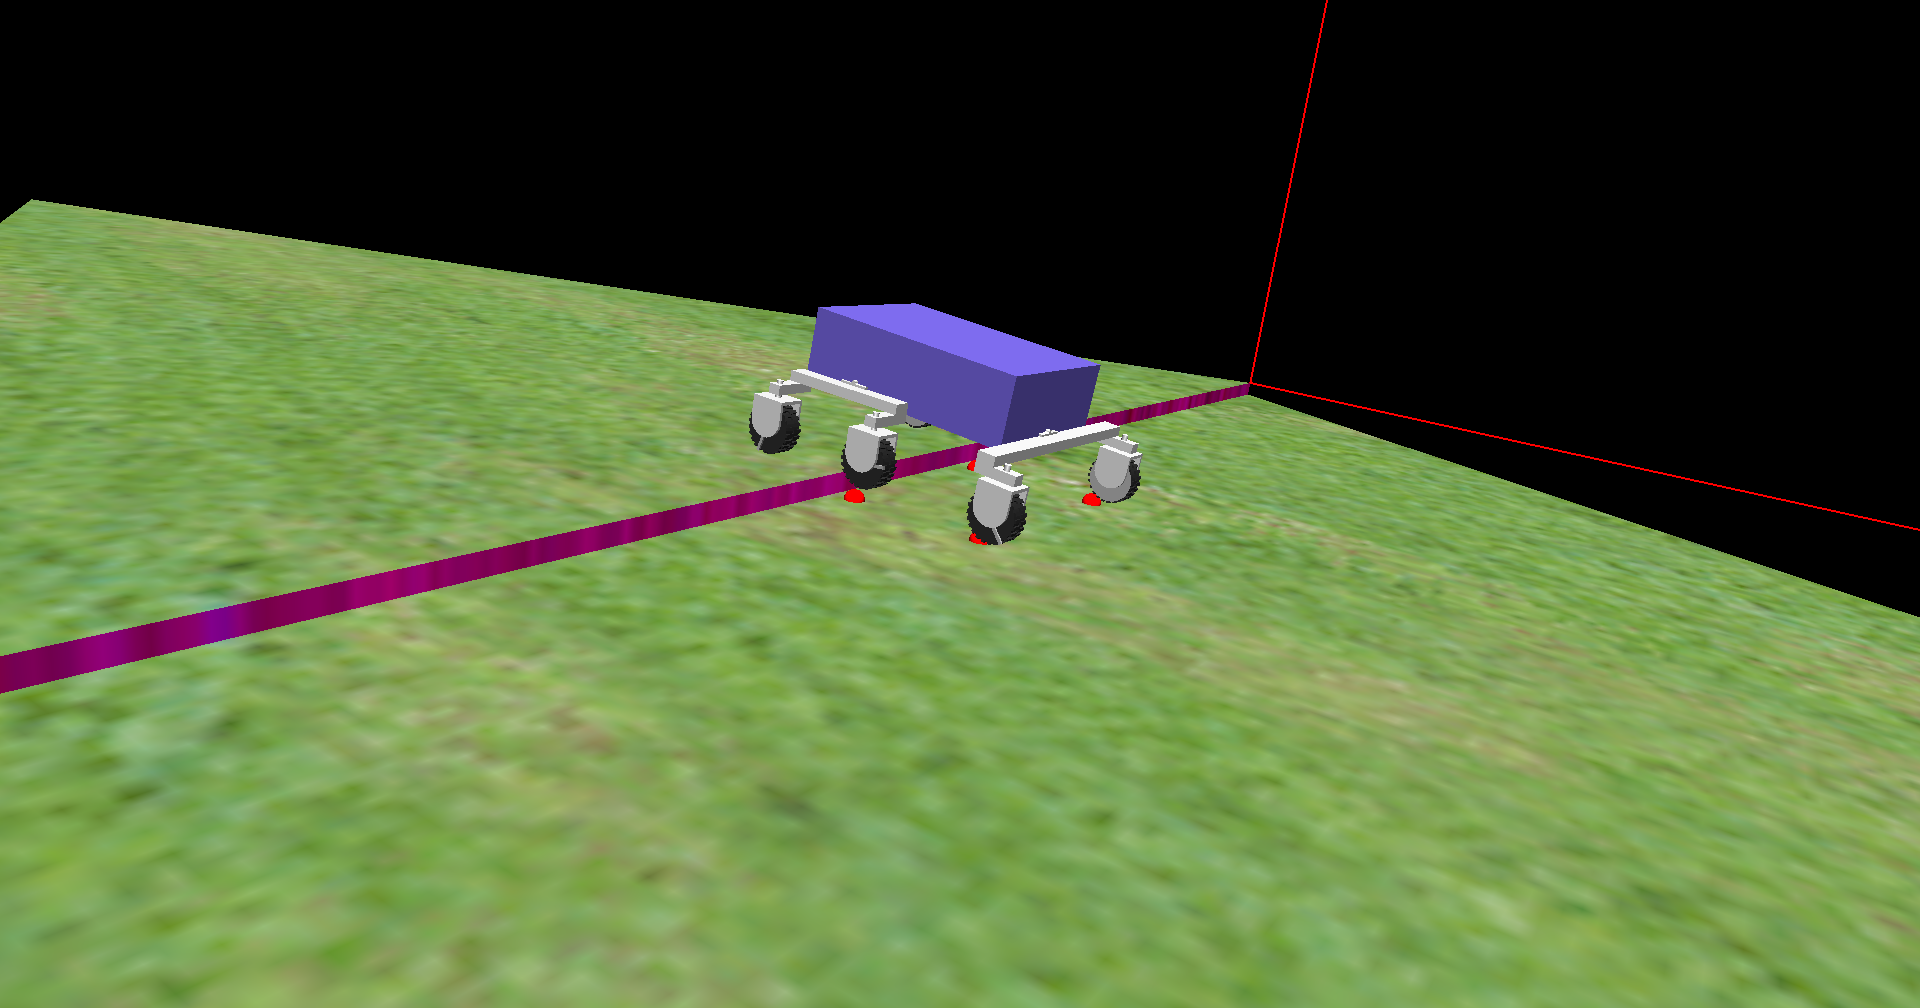
\includegraphics[width=0.8\textwidth]{run_7}
  \caption{Seventh test scenario}
\end{figure}

\noindent In this case, following quantities have been plotted:

\begin{itemize}
  \item $x_{COM}$ - mass center coordinates
\end{itemize}

\begin{figure}[H]
  \centering
    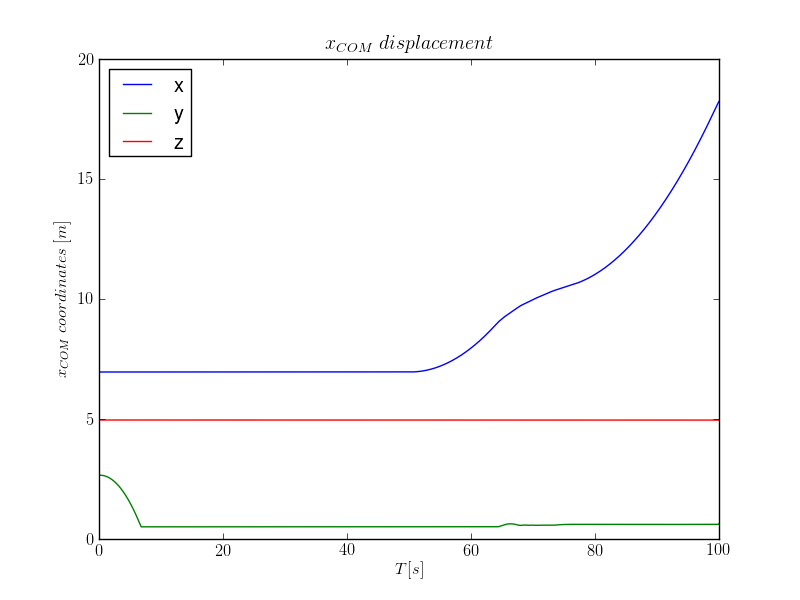
\includegraphics[width=0.8\textwidth]{xCOM7}
  \caption{$x_{COM}$}
\end{figure}

\begin{itemize}
  \item $x_{wheels}$ - wheels angular displacement 
\end{itemize}

\begin{figure}[H]
  \centering
    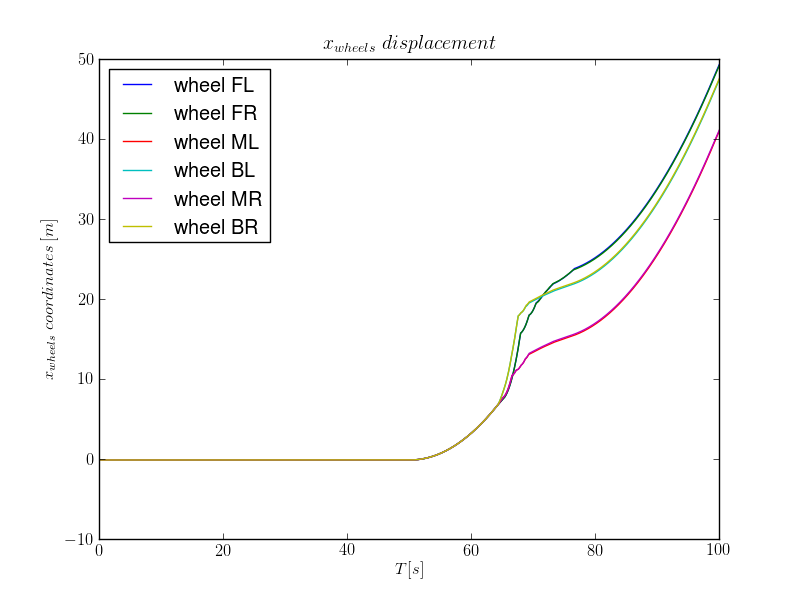
\includegraphics[width=0.8\textwidth]{xWHEELS7}
  \caption{$x_{wheels}$}
\end{figure}

\begin{itemize}
  \item $v_{COM}$ - mass center velocity
\end{itemize}

\begin{figure}[H]
  \centering
    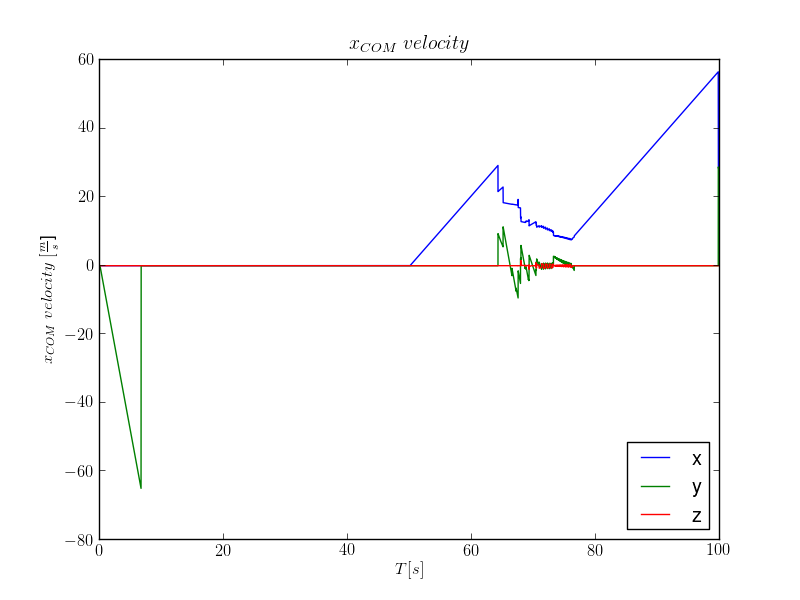
\includegraphics[width=0.8\textwidth]{vCOM7}
  \caption{$v_{COM}$}
\end{figure}

\begin{itemize}
  \item $v_{wheels}$ - wheels angular velocity
\end{itemize}

\begin{figure}[H]
  \centering
    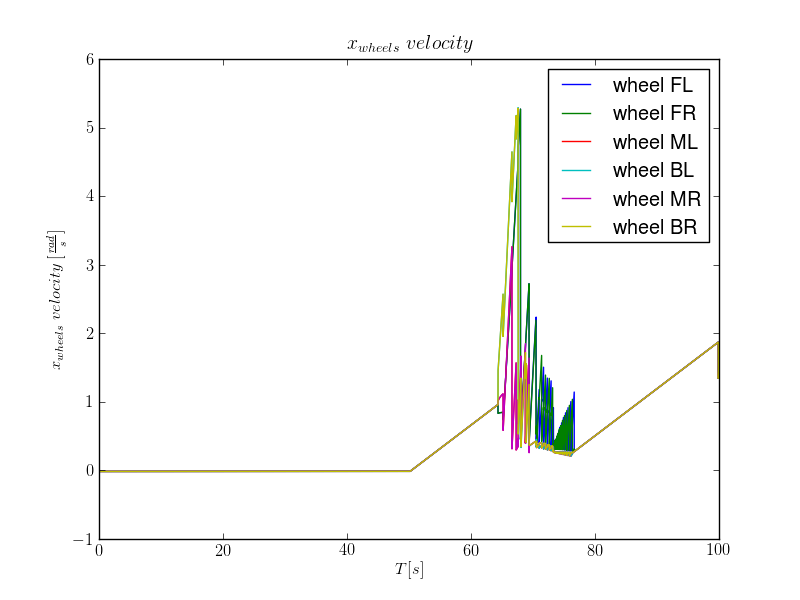
\includegraphics[width=0.8\textwidth]{vWHEELS7}
  \caption{$v_{wheels}$}
\end{figure}

\begin{itemize}
  \item $R_{COM}$ - reaction forces of center of mass in lagrangian coordinates
\end{itemize}

\begin{figure}[H]
  \centering
    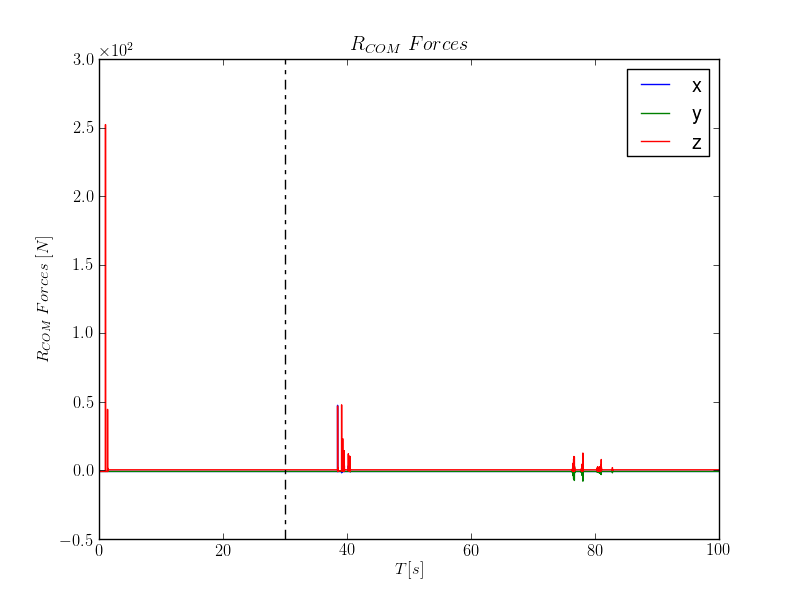
\includegraphics[width=0.8\textwidth]{pCOM7}
  \caption{$R_{COM}$}
\end{figure}

\begin{itemize}
  \item $R_{wheels}$ - reaction forces of wheels in lagrangian coordinates
\end{itemize}

\begin{figure}[H]
  \centering
    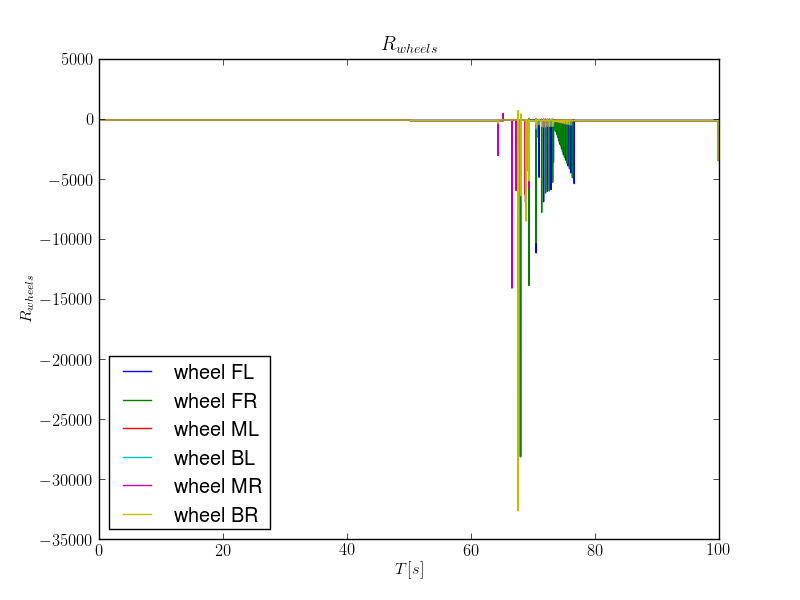
\includegraphics[width=0.8\textwidth]{pWHEELS7}
  \caption{$R_{wheels}$}
\end{figure}
